\documentclass[a4paper,12pt]{article}
\usepackage[left=2cm,right=2cm,top=2cm,bottom=2cm]{geometry} % Do ustawień marginesów
\usepackage{multicol} % Dla podziału na kolumny
\usepackage{ragged2e} % Dla justowania tekstu
\usepackage{graphicx} % Required for inserting images
\usepackage{float}
\usepackage{caption}
\usepackage{amsmath} % Math formulas
\usepackage{amssymb} % Symbols
\usepackage[svgnames]{xcolor}
\usepackage[colorlinks=true, urlcolor=blue, linkcolor=black, citecolor=orange]{hyperref} % Hyperlinks
\usepackage{polski} % Polish language
\usepackage[utf8]{inputenc} % Text encoding
\usepackage{enumitem} % Pakiet do elastycznego sterowania listami
\usepackage{indentfirst}
\usepackage{array}
\usepackage{longtable}
\usepackage{siunitx}

\setlist[itemize]{itemsep=0pt, topsep=0pt}

\begin{document}

% Górna część strony
\noindent
\begin{minipage}{0.5\textwidth}
    \raggedright
    \textbf{Piotr Durniat} \\
    I rok, Fizyka \\
    Wtorek, 8:00-10:15 \\
    \vspace{0.5cm}
    \vspace{0.5cm}
\end{minipage}%
\begin{minipage}{0.5\textwidth}
    \raggedleft
    Data wykonania pomiarów: \\
    06.05.2025 \\
    \vspace{0.5cm}
    Prowadząca: \\
    dr Iwona Mróz
\end{minipage}

% Tytuł ćwiczenia
\vspace{2cm}
\begin{center}
    \LARGE \textbf{Ćwiczenie nr 29} \\[0.5cm]
    \Large \textbf{Anomalia rozszerzalności cieplnej wody}
\end{center}

\vspace{1cm}
\noindent

\tableofcontents
\newpage

% ---------- WSTĘP TEORETYCZNY ----------
\section{Wstęp teoretyczny}

Większość ciał zmienia swoją objętość liniowo wraz z temperaturą zgodnie z równaniem:
\begin{equation}
    V = V_0(1 + \beta T)
\end{equation}
gdzie $V$ to objętość w temperaturze $T$ (w °C), $V_0$ to objętość w 0°C, a $\beta$ to współczynnik rozszerzalności objętościowej, który zależy od rodzaju substancji i stanu skupienia.

W cząsteczkach występują różne rodzaje wiązań atomowych:
\begin{itemize}
    \item wiązania kowalencyjne - powstają przez nakładanie się orbitali atomowych
    \item wiązania jonowe - między jonami dodatnimi i ujemnymi
    \item wiązania wodorowe - szczególnie istotne w przypadku wody
\end{itemize}

Cząsteczka wody (H$_2$O) jest dipolem, gdzie atomy wodoru mają ładunek dodatni, a atom tlenu ujemny. Wiązania OH tworzą kąt 104{,}5°, co jest spowodowane polarnością wiązań. W stanie ciekłym cząsteczki wody łączą się wiązaniami wodorowymi, tworząc strukturę przypominającą kryształ z bliskim porządkiem.

Woda zachowuje się nietypowo w zakresie temperatur 0-4°C. Powyżej 4°C jej objętość maleje wraz z obniżaniem temperatury, jak u większości ciał. Jednak w zakresie 0-4°C objętość wody rośnie przy ochładzaniu, osiągając minimum (a więc maksymalną gęstość) w temperaturze 4°C. To zjawisko nazywamy anomalną rozszerzalnością cieplną wody.

Poniżej 4°C cząsteczki wody intensywnie asocjują, tworząc heksagonalną strukturę podobną do lodu. Ta struktura ma duże, otwarte przestrzenie, co prowadzi do zmniejszenia gęstości (około 0,9 g/cm$^3$ dla lodu). Podczas topnienia wiązania wodorowe pękają, pozwalając cząsteczkom na ciaśniejsze ułożenie, co powoduje zmniejszenie objętości o około 10\% względem fazy ciekłej.

Ta anomalia ma istotne znaczenie ekologiczne - zimą woda o temperaturze 4°C opada na dno zbiornika, podczas gdy zimniejsza unosi się do góry i zamarza na powierzchni. Lód izoluje zbiornik, a woda przy dnie pozostaje w okolicach 4°C, umożliwiając przetrwanie organizmów wodnych.

Wstęp teoretyczny opracowano na podstawie następujących źródeł: podręcznika \cite{fizyka_dla_szkół_wyższych_tom_2}, który zawiera podstawowe informacje o rozszerzalności cieplnej ciał, oraz wstępu do ćwiczenia \cite{lab29manual}.

% ---------- OPIS DOŚWIADCZENIA ----------
\section{Opis doświadczenia}

Doświadczenie polegało na badaniu zmiany objętości wody w funkcji temperatury. Wykonano je w następujących etapach:

\begin{itemize}
    \item Przygotowano aparaturę pomiarową składającą się z:
          \begin{itemize}
              \item kolby z wodą destylowaną ($V_{\text{kolby}} = 300\,\text{cm}^3$)
              \item kapilary o średnicy wewnętrznej $d = 1{,}7\,\text{mm}$
              \item termometru elektronicznego o dokładności $0{,}1^\circ$C
              \item mieszadła magnetycznego
          \end{itemize}

    \item Przeprowadzono pomiary w dwóch seriach:
          \begin{itemize}
              \item ochładzanie: od $11^\circ$C do $0{,}3^\circ$C (co $0{,}2^\circ$C)
              \item ogrzewanie: od $0{,}3^\circ$C do $11^\circ$C (co $0{,}2^\circ$C)
          \end{itemize}

    \item Dla każdej temperatury zmierzono wysokość słupa wody w kapilarze

    \item Na podstawie pomiarów obliczono:
          \begin{itemize}
              \item objętość wody w kapilarze
              \item całkowitą objętość wody
              \item zmianę objętości względem minimalnej
              \item względną zmianę gęstości
          \end{itemize}
\end{itemize}

% ---------- OPRACOWANIE WYNIKÓW POMIARÓW ----------
\section{Opracowanie wyników pomiarów}

% ---------- TABELE ----------
\subsection{Tabele pomiarowe}

\begin{table}[H]
    \centering
    \begin{minipage}{0.48\textwidth}
        \centering
        \begin{tabular}{|c|c|c|}
            \hline
            $T$ [$^\circ$C] & \multicolumn{2}{c|}{$h$ [mm]} \\
            \hline
            & Seria 1 & Seria 2 \\
            \hline
            11{,}0 & 80 & 71 \\
            10{,}8 & 77 & 70 \\
            10{,}6 & 75 & 68 \\
            10{,}4 & 74 & 66 \\
            10{,}2 & 72 & 64 \\
            10{,}0 & 69 & 62 \\
            9{,}8  & 68 & 60 \\
            9{,}6  & 66 & 58 \\
            9{,}4  & 64 & 56 \\
            9{,}2  & 63 & 55 \\
            9{,}0  & 61 & 54 \\
            8{,}8  & 61 & 51 \\
            8{,}6  & 60 & 51 \\
            8{,}4  & 56 & 49 \\
            8{,}2  & 55 & 48 \\
            8{,}0  & 53 & 46 \\
            7{,}8  & 52 & 44 \\
            7{,}6  & 51 & 44 \\
            7{,}4  & 50 & 43 \\
            7{,}2  & 49 & 41 \\
            7{,}0  & 47 & 40 \\
            6{,}8  & 46 & 39 \\
            6{,}6  & 45 & 37 \\
            6{,}4  & 44 & 37 \\
            6{,}2  & 43 & 36 \\
            6{,}0  & 42 & 40 \\
            5{,}8  & 42 & 36 \\
            5{,}6  & 42 & 34 \\
            5{,}4  & 40 & 32 \\
            5{,}2  & 40 & 32 \\
            5{,}0  & 39 & $<30$ \\
            \hline
        \end{tabular}
    \end{minipage}
    \hfill
    \begin{minipage}{0.48\textwidth}
        \centering
        \begin{tabular}{|c|c|c|}
            \hline
            $T$ [$^\circ$C] & \multicolumn{2}{c|}{$h$ [mm]} \\
            \hline
            & Seria 1 & Seria 2 \\
            \hline
            4{,}8  & 38 & $<30$ \\
            4{,}6  & 38 & $<30$ \\
            4{,}4  & 38 & $<30$ \\
            4{,}2  & 37 & $<30$ \\
            4{,}0  & 37 & $<30$ \\
            3{,}8  & 37 & $<30$ \\
            3{,}6  & 37 & $<30$ \\
            3{,}4  & 37 & $<30$ \\
            3{,}2  & 37 & $<30$ \\
            3{,}0  & 37 & $<30$ \\
            2{,}8  & 37 & 30 \\
            2{,}6  & 37 & 30 \\
            2{,}4  & 38 & 30 \\
            2{,}2  & 38 & 32 \\
            2{,}0  & 38 & 33 \\
            1{,}8  & 39 & 34 \\
            1{,}6  & 39 & 34 \\
            1{,}4  & 40 & 35 \\
            1{,}2  & 40 & 36 \\
            1{,}0  & 41 & 37 \\
            0{,}8  & 41 & 38 \\
            0{,}6  & 42 & 39 \\
            0{,}4  & 43 & 40 \\
            0{,}2  & 43 & 41 \\
            \hline
        \end{tabular}
    \end{minipage}
    \caption{Wyniki pomiarów wysokości słupa wody w zależności od temperatury}
    \label{tab:pomiary_wysokosci}
\end{table}

Średnica wewnętrzna kapilary wynosi $d = 1{,}7\,\text{mm}$.

Do obliczeń wybrano serię 1, gdyż w drugiej serii doszło do przesunięcia poziomu wody w kapilarze względem serii pierwszej, oraz ze względu na wyjście poniżej wartości 30°C nie było możliwości dokładnego pomiaru.

% ---------- OBLICZENIA ----------
\subsection{Zmiana objętości wody}

Na podstawie zmierzonej wysokości słupa wody obliczono objętość wody w kapilarze według wzoru:
\begin{equation}
    V = V_{\text{kolby}} +\pi \cdot \frac{d^2}{4} \cdot h
\end{equation}

gdzie $d = 1{,}7\,\text{mm}$ jest średnicą wewnętrzną kapilary, a $h$ jest wysokością słupa wody, $V_{\text{kolby}} = 300 \cdot 10^{-6}\,\text{m}^3$ jest objętością kolby.

Obliczono również zmianę objętości $\Delta V$ względem objętości minimalnej (dla temperatury 4°C):
\begin{equation}
    \Delta V = V - V_{4^\circ C}
\end{equation}

\begin{table}[H]
    \centering
    \caption{Wartości objętości wody oraz zmiany objętości (wybrane temperatury)}
    \label{tab:objetosci}
    \begin{tabular}{|c|c|c|c|c|}
        \hline
        $T$ [$^\circ$C] & $V_1$ [m$^3$] & $V_2$ [m$^3$] & $\Delta V_1$ [m$^3$] & $\Delta V_2$ [m$^3$] \\
        \hline
        11{,}0 & 3{,}0018$\cdot$10$^{-4}$ & 3{,}0016$\cdot$10$^{-4}$ & 9{,}76$\cdot$10$^{-8}$ & 9{,}31$\cdot$10$^{-8}$ \\
        10{,}0 & 3{,}0016$\cdot$10$^{-4}$ & 3{,}0014$\cdot$10$^{-4}$ & 7{,}26$\cdot$10$^{-8}$ & 7{,}26$\cdot$10$^{-8}$ \\
        9{,}0 & 3{,}0014$\cdot$10$^{-4}$ & 3{,}0012$\cdot$10$^{-4}$ & 5{,}45$\cdot$10$^{-8}$ & 5{,}45$\cdot$10$^{-8}$ \\
        8{,}0 & 3{,}0012$\cdot$10$^{-4}$ & 3{,}0010$\cdot$10$^{-4}$ & 3{,}63$\cdot$10$^{-8}$ & 3{,}63$\cdot$10$^{-8}$ \\
        7{,}0 & 3{,}0011$\cdot$10$^{-4}$ & 3{,}0009$\cdot$10$^{-4}$ & 2{,}27$\cdot$10$^{-8}$ & 2{,}27$\cdot$10$^{-8}$ \\
        6{,}0 & 3{,}0010$\cdot$10$^{-4}$ & 3{,}0008$\cdot$10$^{-4}$ & 1{,}36$\cdot$10$^{-8}$ & 1{,}36$\cdot$10$^{-8}$ \\
        5{,}0 & 3{,}0009$\cdot$10$^{-4}$ & 3{,}0007$\cdot$10$^{-4}$ & 4{,}54$\cdot$10$^{-9}$ & 4{,}54$\cdot$10$^{-9}$ \\
        4{,}0 & 3{,}0008$\cdot$10$^{-4}$ & 3{,}0007$\cdot$10$^{-4}$ & 0{,}00$\cdot$10$^{-8}$ & 0{,}00$\cdot$10$^{-8}$ \\
        3{,}0 & 3{,}0008$\cdot$10$^{-4}$ & 3{,}0007$\cdot$10$^{-4}$ & 2{,}27$\cdot$10$^{-9}$ & 4{,}54$\cdot$10$^{-9}$ \\
        2{,}0 & 3{,}0009$\cdot$10$^{-4}$ & 3{,}0007$\cdot$10$^{-4}$ & 4{,}54$\cdot$10$^{-9}$ & 9{,}08$\cdot$10$^{-9}$ \\
        1{,}0 & 3{,}0009$\cdot$10$^{-4}$ & 3{,}0008$\cdot$10$^{-4}$ & 6{,}81$\cdot$10$^{-9}$ & 1{,}13$\cdot$10$^{-8}$ \\
        0{,}2 & 3{,}0010$\cdot$10$^{-4}$ & 3{,}0009$\cdot$10$^{-4}$ & 9{,}08$\cdot$10$^{-9}$ & 1{,}36$\cdot$10$^{-8}$ \\
        \hline
    \end{tabular}
\end{table}

Pełne dane objętości dla wszystkich pomiarów przedstawiono na wykresie (Rys.~\ref{fig:height_vs_temperature}). Można zauważyć, że woda osiąga najmniejszą objętość (największą gęstość) w okolicy temperatury 4°C, co potwierdza zjawisko anomalii rozszerzalności cieplnej wody.

\subsection{Względna zmiana gęstości}

Względna zmiana gęstości wody w temperaturze $10^\circ$C względem maksymalnej gęstości. Na podstawie wykresu (Rys.~\ref{fig:height_vs_temperature}) woda osiąga największą gęstość w temperaturze 4°C.

\begin{align*}
     & V_{10^\circ C} = 300 \cdot 10^{-6} + \frac{\pi \cdot 0{,}0017^2 \cdot 0{,}037}{4} = 0{,}00030008\,\text{m}^3                                        \\
     & V_{4^\circ C} = 300 \cdot 10^{-6} + \frac{\pi \cdot 0{,}0017^2 \cdot 0{,}069}{4} = 0{,}0003001\,\text{m}^3                                          \\
     & \frac{\rho(T=4^\circ C) - \rho(T=10^\circ C)}{\rho_{T=4^\circ C}} = \frac{\frac{m}{V(4^\circ C)} - \frac{m}{V(10^\circ C)}}{\frac{m}{V(4^\circ C)}} \\
     & = \frac{V_{10^\circ C} - V_{4^\circ C}}{V_{10^\circ C}} = \frac{0{,}0003001 - 0{,}00030008}{0{,}0003001} = 0{,}00024 = 2{,}4 \cdot 10^{-4}
\end{align*}

% ---------- NIEPEWNOŚCI ----------
\section{Ocena niepewności pomiarowych}

\subsection{Niepewność pomiaru temperatury}

Do pomiaru temperatury użyto termometru elektronicznego o niepewności maksymalnej $\Delta_d T = 0{,}1^\circ$C. Niepewność standardową oszacowano za pomocą metody typu B:

\begin{equation}
    u(t) = \frac{\Delta_d T}{\sqrt{3}} = \frac{0{,}1}{\sqrt{3}} \approx 0{,}0577\,\text{°C}
\end{equation}

\subsection{Niepewność pomiaru wysokości słupa cieczy}

Wysokość słupa wody w kapilarze była odczytywana z niepewnością maksymalną $\Delta_d h = 0{,}001\,\text{m}$. Niepewność standardową oszacowano za pomocą metody typu B:

\begin{equation}
    u(h) = \frac{\Delta h}{\sqrt{3}} = \frac{0{,}001}{\sqrt{3}} \approx 0{,}00058\,\text{m}
\end{equation}

Wykres razem z niepewnościami przedstawiono na Rys.~\ref{fig:height_vs_temperature_with_uncertainties}.

% ---------- WNIOSKI ----------
\section{Wnioski}

\begin{itemize}
    \item Woda osiąga maksymalną gęstość w temperaturze $4^\circ$C, co potwierdza zjawisko anomalii rozszerzalności cieplnej wody \cite{fizyka_dla_szkół_wyższych_tom_2}.

    \item Względna zmiana gęstości wody między temperaturą $10^\circ$C a $4^\circ$C wynosi:
          \[
              \frac{\Delta \rho}{\rho} = 2{,}43 \cdot 10^{-4}
          \]

    \item Niepewność pomiaru wysokości słupa wody wynosi $u(h) = 0{,}00058\,\text{m}$, a niepewność pomiaru temperatury wynosi $u(t) = 0{,}0577\,\text{°C}$.

    \item Wyniki pomiarów potwierdzają, że woda zachowuje się nietypowo w zakresie temperatur $0-4^\circ$C, zwiększając swoją objętość wraz ze spadkiem temperatury.
\end{itemize}

\newpage
% ---------- WYKRESY ----------
\section{Wykresy}

\begin{figure}[H]
    \centering
    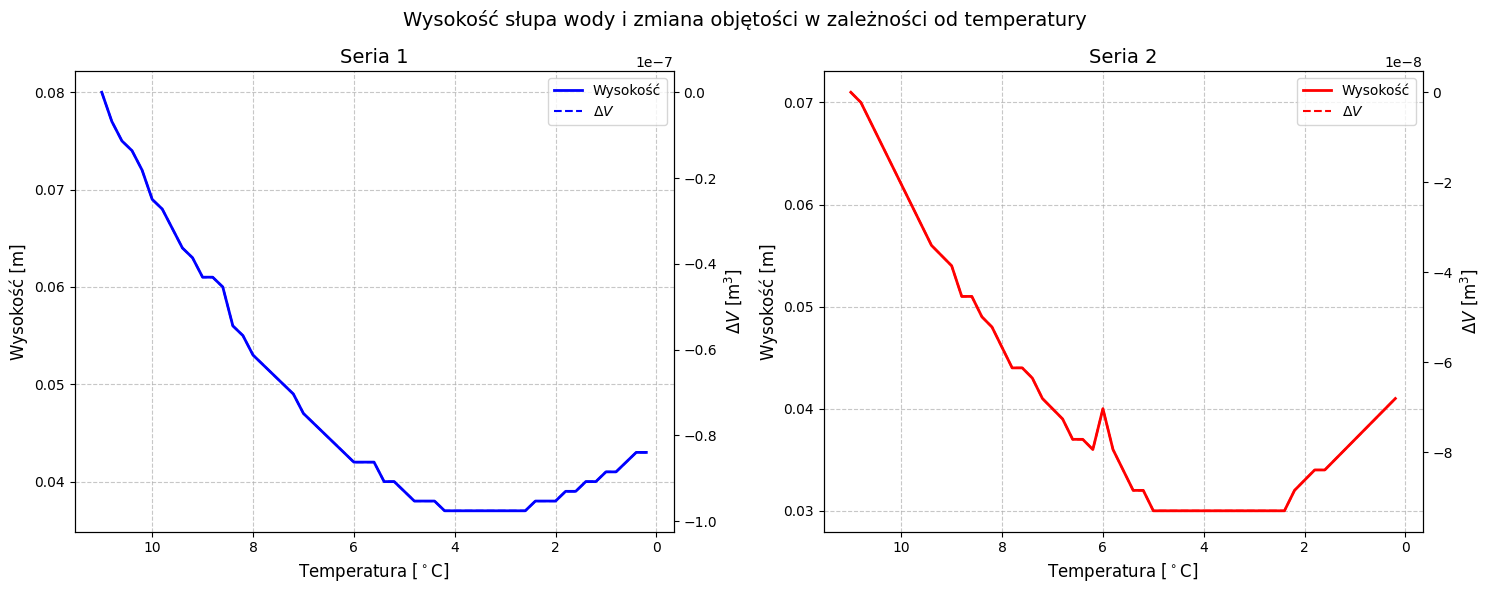
\includegraphics[width=0.9\textheight,angle=90]{height_vs_temperature.png}
    \caption{Wysokość słupa wody oraz zmiana objętości wody w zależności od temperatury.}
    \label{fig:height_vs_temperature}
\end{figure}

\begin{figure}[H]
    \centering
    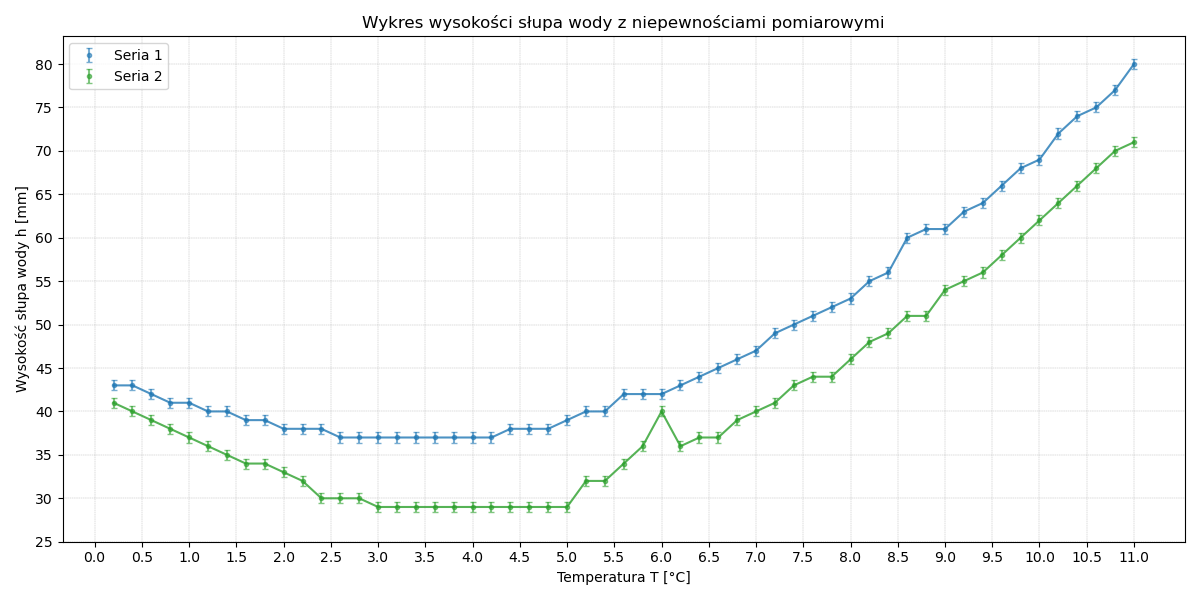
\includegraphics[width=0.9\textheight,angle=90]{height_vs_temperature_uncertainties.png}
    \caption{Wysokość słupa wody oraz zmiana objętości wody w zależności od temperatury z uwzględnieniem niepewności.}
    \label{fig:height_vs_temperature_with_uncertainties}
\end{figure}

\bibliographystyle{plain}
\bibliography{bibliography}

\end{document}
